%
% STAT 100: Chance and Data Analysis - A Course Overview
%
% Author: Jeffrey Leung
%

\documentclass[10pt, oneside, letterpaper, titlepage]{article}

\usepackage[justification=centering]{caption}
\usepackage[ampersand]{easylist}
	\ListProperties(
		Progressive*=5ex,
		Space=5pt,
		Space*=5pt,
		Style1*=\textbullet\ \ ,
		Style2*=\begin{normalfont}\begin{bfseries}\textendash\end{bfseries}\end{normalfont} \ \ ,
		Style3*=\textasteriskcentered\ \ ,
		Style4*=\textperiodcentered\ \ ,
		Style5*=\textbullet\ \ ,
		Style6*=\begin{normalfont}\begin{bfseries}\textendash\end{bfseries}\end{normalfont}\ \ ,
		Style7*=\textasteriskcentered\ \ ,
		Style8*=\textperiodcentered\ \ ,
		Hide1=1,
		Hide2=2,
		Hide3=3,
		Hide4=4,
		Hide5=5,
		Hide6=6,
		Hide7=7,
		Hide8=8 )
\usepackage[T1]{fontenc}
\usepackage{geometry}
	\geometry{margin=1.2in}
\usepackage{graphicx}
	\graphicspath{ {img/} }
\usepackage[colorlinks=true, linkcolor=blue]{hyperref}
\usepackage[retainorgcmds]{IEEEtrantools}
\usepackage{lmodern} % Allows the use of symbols in font size 10; http://ctan.org/pkg/lm
\usepackage{multirow}
\usepackage{pgfplots, pgfplotstable}
	\usepgfplotslibrary{statistics}
	\pgfplotsset{compat=newest}
\usepackage{textcomp} % Allows the use of \textbullet with the font
\usepackage{tikz}
	\usetikzlibrary{patterns}
\usepackage{verbatim}

\renewcommand{\arraystretch}{1.2}
\renewcommand{\familydefault}{\sfdefault}

\title{STAT 100: Chance and Data Analysis \\\medskip \Large A Course Overview}
\author{Jeffrey Leung \\ Simon Fraser University}
\date{Fall 2015}

\begin{document}

	\maketitle
	\tableofcontents
	\clearpage
	
	%
% STAT 100: Chance and Data Analysis - A Course Overview
% Section: Elements of Statistics
%
% Author: Jeffrey Leung
%

\section{Elements of Statistics}
	\label{sec:elements-of-statistics}
\subsection{Subject of Study}
	\label{subsec:elements-of-statistics:subject-of-study}
\begin{easylist}

	& \emph{Statistics:} Collection, organization, analysis, and interpretation of data
		&& \emph{Statistic:} Number which summarizes data about a sample
		&& \emph{Descriptive statistic:} Description or summary about a sample
			&&& Often inferred from analyzed statistics
		&& \emph{Parameter:} Value which summarizes data about a population
			&&& Calculated exactly by collecting data from the entire population (see \emph{census}, subsection~ %TODO reference, and 'exactly'?
			&&& Estimated by calculating a statistic about a representative sample of the population
			
	
	\bigskip
	
	& \emph{Individual:} Object of study about which data is collected
		&& Not necessarily a person
	& \emph{Sample:} Individual from which data is collected directly
		&& See \emph{sample survey}, subsection~\ref{subsec:data-collection:methods}
	& \emph{Population:} Set of \emph{all} individuals for which data is inferred
		&& Inference about the population is made from the data of the sample
		&& See \emph{census}, subsection~\ref{subsec:data-collection:methods}
	
	\medskip	
	
	& Example: In an analysis of salary distribution of all UBC recent graduates, a research team collected information from 500 individuals. The data contained the annual salary, age, occupation, gender, and year of graduation of the individual. \smallskip \\
	Individual: A UBC recent graduate \\
	Sample: The 500 surveyed UBC recent graduates \\
	Population: All UBC recent graduates
		
\end{easylist}
\subsection{Categorical Variables}
	\label{subsec:elements-of-statistics:categorical-variables}
\begin{easylist}

	& \emph{Variable:} Data collected from an individual
	
	& \emph{Categorical:} Variable which is a label or category
		&& Example: Occupation, gender
		&& Has no unit of measurement
		&& All possible options must be specified
		&& Statistics of categorical data are the percentages/proportions of all categories
		&& Displayed using a bar graph
	
	& Example: A study is conducted to collect the following information from an SFU student.
		&& Whether or not an SFU student has a profile on Facebook \\
			(categorical variable - options are yes or no)
		&& Number of text messages sent recently \\
			(not a categorial variable - number, not specific options)
		&& How long it took to download the most recent video game \\
			(not a categorical variable - amount, not specific options)
			
	& For the analysis of categorical data, see subsection~\ref{subsec:analysis-of-single-variable-data:categorical-data}
	& For an example with both quantitative and categorical variables, see \emph{Quantitative Variables}, subsection~\ref{subsec:elements-of-statistics:quantitative-variables}
	
\end{easylist}
\subsection{Quantitative Variables}
	\label{subsec:elements-of-statistics:quantitative-variables}
\begin{easylist}
		
	& See \emph{variable}, subsection~\ref{subsec:elements-of-statistics:categorical-variables}
	
	& \emph{Quantitative:} Variable which is countable
		&& E.g. Salary, age
		&& Always has a unit of measurement
		&& Can have basic mathematical operations applied to it
		&& Examples of quantitative statistics:
			&&& Average/mean
			&&& Median
			&&& Standard deviation
			&&& Quartiles
			&&& Maximum/minimum
		&& Displayed using a histogram
	
	\medskip
	& Example: A study is conducted to collect the following information from an SFU student.
		&& Whether or not an SFU student has a profile on Facebook \\
			(not a quantitative variable - not a number)
		&& Number of text messages sent recently \\
			(quantitative variable - number of messages)
		&& How long it took to download the most recent video game \\
			(quantitative variable - amount of time)
			
	& For the analysis of quantitative data, see subsection~\ref{subsec:analysis-of-single-variable-data:quantitative-data}
	
	& Example: 7 countries were studied; the results are shown in table~\ref{tab:information-gathered-on-7-countries}.
	
	\Deactivate
	\begin{table}[!htb]
		\centering
		\caption{Information gathered on 7 Countries}
		\label{tab:information-gathered-on-7-countries}
		\begin{tabular}{ l | l r r r }
			& & Land area & Population & GDP \\
			Country & Continent & (km\textsuperscript{2}) & (millions) & (per capita) \\
			\hline
			Canada & North America & 9,093,510 & 33.31 & 46,236 \\
			China & Asia & 9,327,480 & 1324.66 & 4,428 \\
			Germany & Europe & 348,630 & 82.11 & 40,152 \\
			India & Asia & 2,974,190 & 1,139.97 & 1,475 \\
			Japan & Asia & 364,500 & 127.70 & 42,831 \\
			South Africa & Africa & 1,214,470 & 48.79 & 7,275 \\
			United States & North America & 9,147,420 & 304.38 & 47,199
		\end{tabular}
	\end{table}
	\Activate
	
	\medskip
	Individual: A country in the world \\
	Sample: The 7 countries surveyed \\
	Population: All countries in the world \\
	Quantitative variables: Land area, populations, GDP \\
	Categorical variable: Continent

\end{easylist}
\clearpage
	%
% STAT 100: Chance and Data Analysis - A Course Overview
% Section: Analysis of Single-Variable Data
%
% Author: Jeffrey Leung
%

\section{Analysis of Single-Variable Data}
	\label{sec:analysis-of-single-variable-data}
\subsection{Categorical Data}
	\label{subsec:analysis-of-single-variable-data:categorical-data}
\begin{easylist}	
	
	& Analysis using statistics, tables, and graphs:
		&& Identify all options for the categorical variable(s)
		&& Create a frequency table
			&&& Total the number of each option chosen
			&&& Use a two-way frequency table if necessary (see \emph{Two-way frequency table}, below)
		&& Calculate the percentage/proportion of each category
			&&& $\frac{frequency}{total\ sample\ size}$
		&& Use graphs to visually display the data
			&&& E.g. Pie chart, line chart, bar graph
		&& Summarize the data and draw conclusions
			&&& Several sentences
			&&& Describe which options are the most/least frequent
			&&& Do not simply reproduce the numbers
		
		\medskip
		&& E.g. A study was conducted on SFU students to determine their opinion (agree/neutral/disagree) on purchasing an iPad as a substitution of textbooks. See table~\ref{tab:ipad-textbook-replacement} for the results.

		\Deactivate
		\begin{table}[!htb]
			\centering
			\caption{Opinions of Students on iPads as Textbook Substitutions}
			\label{tab:ipad-textbook-replacement}
			\begin{tabular}{ r l }
				Student ID & Opinion \\
				\hline
				 1 & Disagree \\
				 2 & Disagree \\
				 3 & Neutral \\
				 4 & Neutral \\
				 5 & Neutral \\
				 6 & Agree \\
				 7 & Disagree \\
				 8 & Neutral \\
				 9 & Disagree \\
				10 & Disagree \\
				11 & Agree \\
				12 & Neutral \\
				13 & Agree \\
				14 & Disagree \\
				15 & Neutral \\
				16 & Neutral \\
				17 & Agree \\
				18 & Disagree \\
				19 & Agree \\
				20 & Neutral
			\end{tabular}
		\end{table}
		\Activate
		
		\smallskip
		Variable: Opinion on purchasing an iPad as a substitution for textbooks \\
		Categories: Agree, neutral, disagree
		
		\smallskip
		For the frequency and percentage table, see table~\ref{tab:ipad-textbook-replacement-freq-table}.
			
		\Deactivate
		\begin{table}[!htb]
			\centering
			\caption{Frequency and Percentage Table of Opinions of Students on iPads as Textbook Substitutions}
			\label{tab:ipad-textbook-replacement-freq-table}
			\begin{tabular}{ l r r }
				Opinion:	& Frequency:	& Percentage: \\
				\hline
				Agree		& 5 			& 25 \\
				Neutral		& 8 			& 40 \\
				Disagree	& 7 			& 35 \\
				\hline
				Total:		& 20			& 100
			\end{tabular}
		\end{table}
		\Activate
		
		\smallskip
		For the bar graph, see figure~\ref{fig:ipad-textbook-replacement-bar-graph}.
		
		\begin{figure}[!htb]
			\centering
			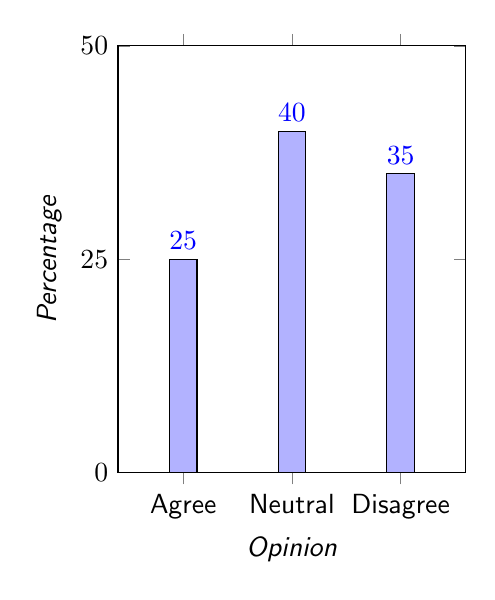
\begin{tikzpicture}
				\begin{axis}
					[
						enlarge x limits=0.3,
						%axis lines*=left, % Removes the top and right borders
						width=6cm,
						height=7cm,
						xtick=data,
						ybar,
						ymin=0,
						ymax=50,
						ytick={0, 25, 50},
						%bar width=\textwidth*.1,
						bar shift=0pt,
						symbolic x coords={Agree, Neutral, Disagree},
						nodes near coords,
						nodes near coords align = vertical,
						xlabel={\emph{Opinion}},
						ylabel={\emph{Percentage}}
					]
					\addplot+
						[
							draw=black
						]
						coordinates
						{
							(Agree, 25)
							(Neutral, 40)
							(Disagree, 35)
						};
				\end{axis}
			\end{tikzpicture}
			
			\caption{Bar Graph of Opinions of Students on iPads as Textbook Substitutions}
			\label{fig:ipad-textbook-replacement-bar-graph}
		\end{figure}
		
		\smallskip
		Conclusion: A large portion of students (40\%) stay neutral on purchasing an iPad as a substitution of textbooks. A small portion of students (25\%) agree on purchasing an iPad as a substitution of textbooks.
	
	& \emph{Two-way frequency table:} Table which allows the comparison of the frequency of two variables
		&& I.e. See table~\ref{tab:freq-table-example}
		
		\Deactivate
		\begin{table}[!htb]
			\centering
			\caption{Example of a two-way frequency table}
			\label{tab:freq-table-example}
			\begin{tabular}{ l l | r r | r }
				\multicolumn{2}{ c | }{} & \multicolumn{2}{ c | }{\emph{Var2}} & \\
				\multicolumn{2}{ c | }{} & Option1 & Option2 & \emph{Total:} \\
				\hline
				\multirow{2}{*}{\emph{Var1}}& Option1 & & & \\
				& Option2 & & & \\
				\hline
				\emph{Total:} & & & & 
			\end{tabular}
		\end{table}
		\Activate
		
		&& \emph{Side-by-side bar chart:} Display of multiple objects of study, each with multiple variable data (all objects sharing the same variables)
			&&& See figure~\ref{fig:side-by-side-bar-chart-example}

			\begin{figure}[!htb]
				\centering
				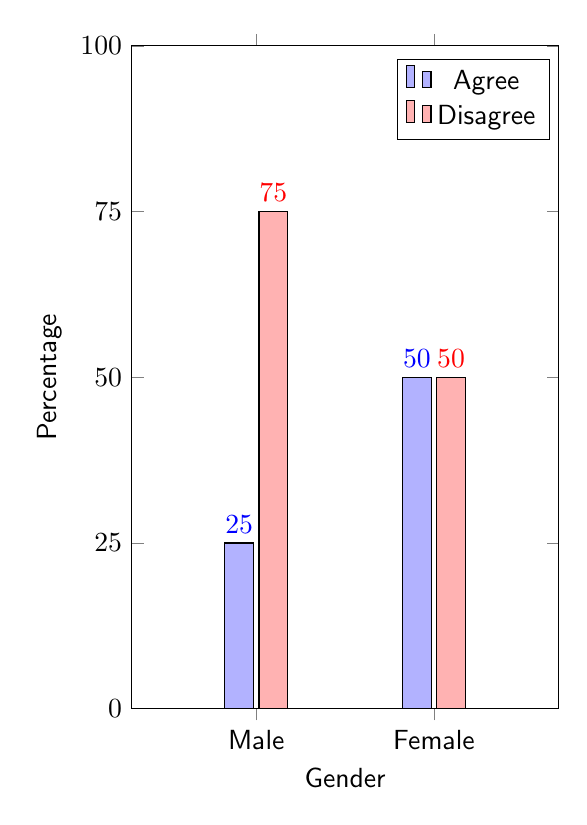
\begin{tikzpicture}
					\begin{axis}
						[
							enlarge x limits=0.7,
							%axis lines*=left, % Removes the top and right borders
							width=7cm,
							height=10cm,
							compat=newest,
							ybar,
							xtick=data,
							ymin=0,
							ymax=100,
							ytick={0, 25, 50, 75, 100},
							bar width=\textwidth*.03,
							symbolic x coords={Male, Female},
							nodes near coords,
							%nodes near coords align = vertical,z
							xlabel={Gender},
							ylabel={Percentage},
						]
						\addplot+
							[
								draw=black
							]
							coordinates
							{
								(Male, 25)
								(Female, 50)
							};
						\addplot+
							[
								draw=black
							]
							coordinates
							{
								(Male, 75)
								(Female, 50)
							};
						\legend{Agree, Disagree}
					\end{axis}
				\end{tikzpicture}
		
				\caption{Distribution of Agreement by Gender}
				\label{fig:side-by-side-bar-chart-example}
			\end{figure}
			
		&& Create $x$ bar charts to isolate analysis of each variable, where $x =$ number of variables per object of study
			&&& Compare the magnitude of the same choice in different sample groups
		
		&& Example: A study was conducted on the distribution of smokers by gender. The results were as follows: \\
		50\% of males smoked; 50\% of males did not smoke. \\
		20\% of females smoked; 80\% of females did not smoke.
		
		\medskip
		For the side-by-side bar graph, see figure~\ref{fig:distribution-of-smokers-by-gender}.
		
		\begin{figure}[!htb]
			\centering
			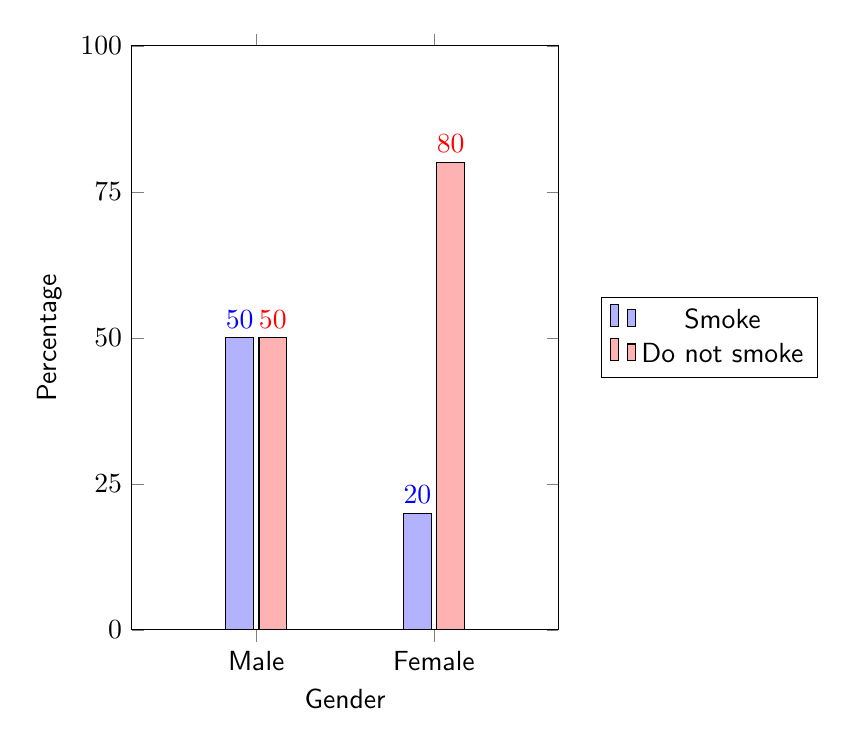
\begin{tikzpicture}
				\begin{axis}
					[
						% GRAPH:
						width=7cm,
						height=9cm,
						%axis lines*=left, % Removes the top and right borders
						% BARS:
						ybar, % Bar chart
						%bar width=\textwidth*.03,
						enlarge x limits=0.7, % Decreases distance between bars
						nodes near coords,
						nodes near coords align = vertical,
						% AXES:
						xtick=data,
						ytick={0, 25, 50, 75, 100},
						symbolic x coords={Male, Female},
						xlabel={Gender},
						ylabel={Percentage},
						ymin=0,
						ymax=100,
						%LEGEND:
						legend style={at={(1.1,0.5)},anchor=west},
					]
					\addplot+
						[
							draw=black
						]
						coordinates
						{
							(Male, 50)
							(Female, 20)
						};
					\addplot+
						[
							draw=black
						]
						coordinates
						{
							(Male, 50)
							(Female, 80)
						};
					\legend{Smoke, Do not smoke}
				\end{axis}
			\end{tikzpicture}
			
			\caption{Distribution of Smokers by Gender}
			\label{fig:distribution-of-smokers-by-gender}
		\end{figure}
		
		From figure~\ref{fig:distribution-of-smokers-by-gender:comparison-of-smokers}, the percentage of smokers is higher in the male group than the female group by 30\%.
		
		\begin{figure}[!htb]
			\centering
			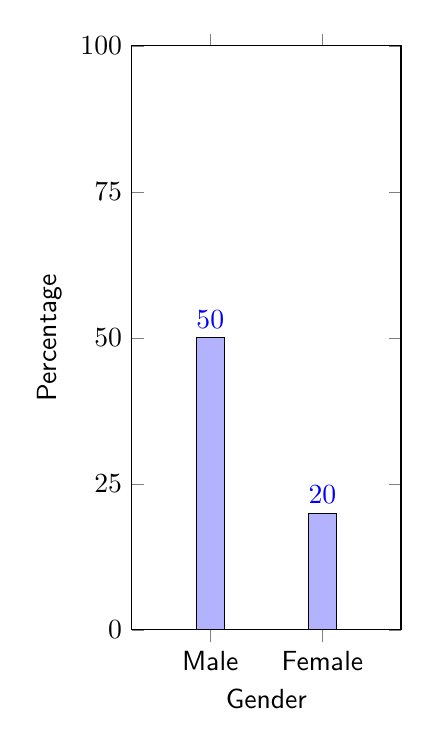
\begin{tikzpicture}
				\begin{axis}
					[
						% GRAPH:
						width=5cm,
						height=9cm,
						%axis lines*=left, % Removes the top and right borders
						% BARS:
						ybar, % Bar chart
						%bar width=\textwidth*.1,
						enlarge x limits=0.7, % Decreases distance between bars
						nodes near coords,
						nodes near coords align = vertical,
						% AXES:
						xtick=data,
						ytick={0, 25, 50, 75, 100},
						symbolic x coords={Male, Female},
						xlabel={Gender},
						ylabel={Percentage},
						ymin=0,
						ymax=100
					]
					\addplot+
						[
							draw=black
						]
						coordinates
						{
							(Male, 50)
							(Female, 20)
						};
				\end{axis}
			\end{tikzpicture}
			
			\caption{Comparison of Male and Female Smokers in a Distribution of Smokers by Gender}
			\label{fig:distribution-of-smokers-by-gender:comparison-of-smokers}
		\end{figure}
		
		From figure~\ref{fig:distribution-of-smokers-by-gender:comparison-of-nonsmokers}, the percentage of nonsmokers is higher in the female group than the male group by 30\%.
		
		\begin{figure}[!htb]
			\centering
			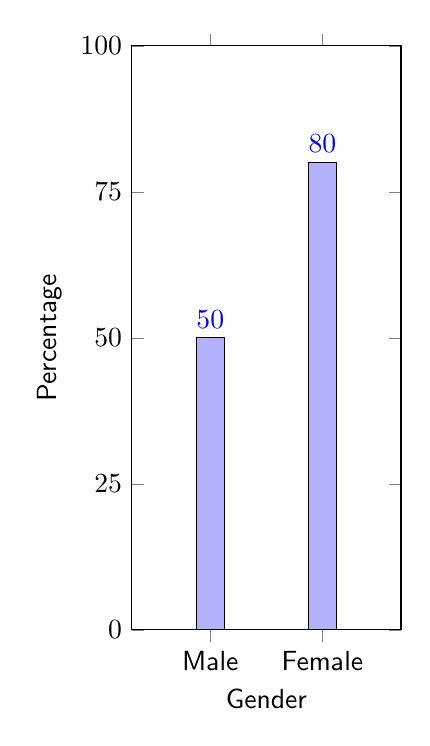
\begin{tikzpicture}
				\begin{axis}
					[
						% GRAPH:
						width=5cm,
						height=9cm,
						%axis lines*=left, % Removes the top and right borders
						% BARS:
						ybar, % Bar chart
						%bar width=\textwidth*.1,
						enlarge x limits=0.7, % Decreases distance between bars
						nodes near coords,
						nodes near coords align = vertical,
						% AXES:
						xtick=data,
						ytick={0, 25, 50, 75, 100},
						symbolic x coords={Male, Female},
						xlabel={Gender},
						ylabel={Percentage},
						ymin=0,
						ymax=100
					]
					\addplot+
						[
							draw=black
						]
						coordinates
						{
							(Male, 50)
							(Female, 80)
						};
				\end{axis}
			\end{tikzpicture}
			
			\caption{Comparison of Male and Female Non-Smokers in a Distribution of Smokers by Gender}
			\label{fig:distribution-of-smokers-by-gender:comparison-of-nonsmokers}
		\end{figure}

\end{easylist}
\subsection{Quantitative Data}
	\label{subsec:analysis-of-single-variable-data:quantitative-data}
\begin{easylist}	

	& Analysis using statistics, tables, and graphs:
		&& Divide the range of data into even classes
			&&& \emph{Class:} Range of values equal in length to all other classes, with no values between classes and no overlapping of classes
				&&&& I.e. Equal-length adjacent ranges of values
				&&&& E.g.  0-10, 10-20, 20-30
				&&&& All data must fall into exactly one class (i.e. there must be no value between classes, and the same value cannot be in multiple classes)
		&& Create a frequency table comparing the number of values in each class (see table~\ref{tab:freq-table-classes})
		
		\Deactivate
		\begin{table}[!htb]
			\centering
			\caption{Frequency Table with Classes}
			\label{tab:freq-table-classes}
			\begin{tabular}{ l r }
				Class Range: & Frequency: \\
				\hline
				$ 0 \leq value < 10$ & 5 \\
				$10 \leq value < 20$ & 4 \\
				$20 \leq value < 30$ & 3 \\
				$30 \leq value < 40$ & 2 \\
				$40 \leq value < 50$ & 1 \\
				\hline
				Total: & 15
			\end{tabular}
		\end{table}
		\Activate
		
		&& Create a histogram:
			&&& \emph{Histogram:} Visual display of classes of values against the frequency of data in each class (see figure~\ref{fig:histogram})
			
			\begin{figure}[!htb]
				\centering
				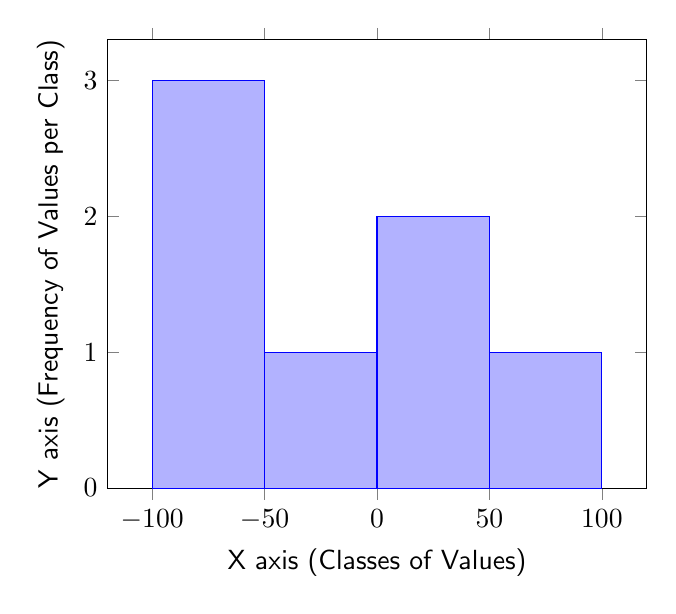
\begin{tikzpicture}[scale=1]
					\begin{axis}
					[
						ybar,
						ymin=0,
						xtick={-100, -50, 0, 50, 100},
						ytick={0, 1, 2, 3},
						xlabel=X axis (Classes of Values),
						ylabel=Y axis (Frequency of Values per Class)
					]
						\addplot +
						[
							hist=
							{
								bins=4,
								data min=-100,
								data max=100
							}
						] table [y index = 0]
						{
							-75
							-75
							-75
							-25
							25
							25
							75
						};
					\end{axis}
				\end{tikzpicture}
				
				\caption{Example of a Histogram}
				\label{fig:histogram}
			\end{figure}
			
			\medskip
			&& E.g. The annual salary (in thousands of dollars) of 10 random UBC graduates was found to be 16, 18, 25, 26, 28, 32, 38, 42, 55, and 80. \smallskip \\
			For the frequency table, see table~\ref{tab:ubc-graduates-salaries-freq-table}.

			\Deactivate
			\begin{table}[!htb]
				\centering
				\caption{Frequency Table of UBC Graduates' Salaries}
				\label{tab:ubc-graduates-salaries-freq-table}
				\begin{tabular}{ l r }
					Classes: & Frequency: \\
					\hline
					$15 \leq salary < 30$ & 5 \\
					$30 \leq salary < 45$ & 3 \\
					$45 \leq salary < 60$ & 1 \\
					$60 \leq salary < 75$ & 0 \\
					$75 \leq salary < 90$ & 1
				\end{tabular}
			\end{table}
			\Activate
			
			For the histogram, see figure~\ref{fig:ubc-graduates-salaries-histogram}.
			
			\begin{figure}[!htb]
				\centering
				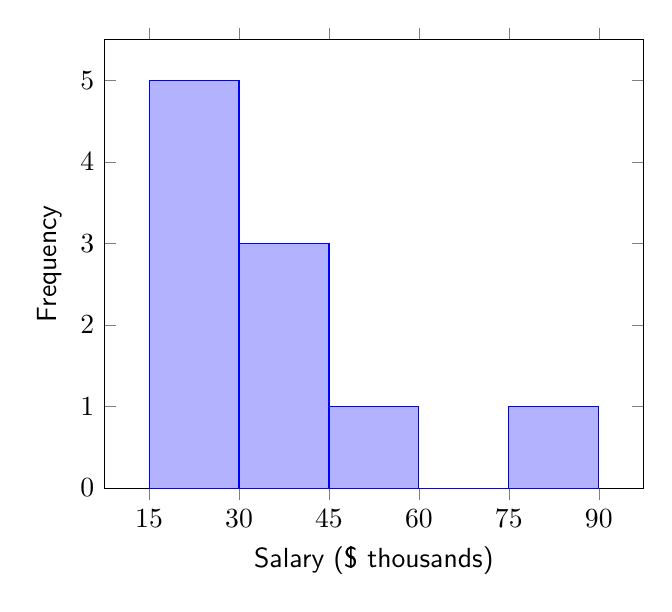
\begin{tikzpicture}[scale=1]
					\begin{axis} %TODO
					[
						ybar,
						ymin=0,
						xtick={15, 30, 45, 60, 75, 90},
						ytick={0, 1, 2, 3, 4, 5},
						xlabel=Salary (\$ thousands),
						ylabel=Frequency
					]
						\addplot +
						[
							hist=
							{
								bins=5,
								data min=15,
								data max=90
							}
						] table [y index = 0]
						{
							16
							18
							25
							26
							28
							32
							38
							42
							55
							80
						};
					\end{axis}
				\end{tikzpicture}
				
				\caption{Histogram of UBC Graduates' Salary}
				\label{fig:ubc-graduates-salaries-histogram}
			\end{figure}

\end{easylist}
\subsection{Statistics of Quantitative Data}
	\label{subsec:analysis-of-single-variable-data:statistics-of-quantitative-data}
\begin{easylist}

	& \emph{Minimum:} Least value in a set of data
	& \emph{Maximum:} Greatest value in a set of data
	& \emph{Range:} Area of values over which the data is spread; expressed in terms of the minimum and maximum
	& \emph{Median:} Number which 50\% of values are less than, and which 50\% of values are greater than
		&& Location in a table of ascending order: $\frac{n + 1}{2}$ where $n =$ the number of data points
			&&& If there are two middle numbers, the median is their average
		&& E.g. The median of values \{1, 3, 5, 7\} is located at $\frac{4+1}{2} = 2.5$. Therefore, the median is the average of the two middle values, which is $\frac{3+5}{2} = 4$.
		&& Example of interpretation: About 50\% of UBC graduates earn less than \$30,000 and the other 50\% of UBC graduates earn greater than \$30,000 per year.
	
	\medskip
	& \emph{Quartiles:} 3 points which divide the data into 4 groups, with the same amount of values in each group
		&& \emph{First quartile (Q1)}: Value which 25\% of the data is less than
			&&& I.e. Median of the lesser half of the data (the median itself is excluded)
		&& \emph{Third quartile (Q3)}: Value which 25\% of the data is greater than
			&&& I.e. Median of the greater half of the data (the median itself is excluded)
		&& Example of interpretation: \\
		About 25\% of UBC graduates earned less than \$25,000. \\
		About 25\% of UBC graduates earned more than \$42,000. \\
		Furthermore, about 50\% of UBC graduates earned between \$25,000 and \$42,000.
	
	\medskip
	& E.g. Given the 11 values \{1, 2, 3, 4, 5, 6, 7, 8, 9, 10, 11\}: (see table~\ref{tab:quantitative-data-statistics-example})
	
	\Deactivate
	\begin{table}[!htb]
		\centering
		\caption{11 Values as an Example of Quantitative Data Statistics}
		\label{tab:quantitative-data-statistics-example}
		\begin{tabular}{ l *{11}{ c } }
			Minimum = 1		& \begin{bfseries} 1 \end{bfseries} & 2 & 3 & 4 & 5 & 6 & 7 & 8 & 9 & 10 & 11 \\
			Maximum = 11	& 1 & 2 & 3 & 4 & 5 & 6 & 7 & 8 & 9 & 10 & \begin{bfseries} 11 \end{bfseries} \\
			Median = 6		& 1 & 2 & 3 & 4 & 5 & \begin{bfseries} 6 \end{bfseries} & 7 & 8 & 9 & 10 & 11 \\
			Q1 = 3			& 1 & 2 & \begin{bfseries} 3 \end{bfseries} & 4 & 5 & 6 & 7 & 8 & 9 & 10 & 11 \\
			Q3 = 9			& 1 & 2 & 3 & 4 & 5 & 6 & 7 & 8 & \begin{bfseries} 9 \end{bfseries} & 10 & 11
		\end{tabular}
	\end{table}
	\Activate
	
	& \emph{Five-number summary:} Description of data using 5 specific values (minimum, first quartile, median, third quartile, maximum)
		&& About 25\% of data falls between:
			&&& The minimum and Q1
			&&& Q1 and the median
			&&& The median and Q3
			&&& Q3 and the maximum
			
		&& \emph{Boxplot:} Visual display of the five-number summary (see figure~\ref{fig:boxplot-example})
			&&& Consists of a box bordered by Q1 and Q3, a vertical line in the box at the median, and two `tails' to the left and right of the box at the minimum and maximum
			
			\begin{figure}[!htb]
				\centering
				\begin{tikzpicture}
					\begin{axis}
					[
						xscale=1.7, % Size of figure
						yscale=.7,
						ytick=0,
						xlabel=X axis
					]
						\addplot+
						[
							boxplot prepared=
							{
								lower whisker=0,
								lower quartile=1,
								median=2,
								upper quartile=3,
								upper whisker=4
							},
						]
						coordinates {} ;
					\end{axis}
				\end{tikzpicture}
				
				\caption{Example of a Boxplot}
				\label{fig:boxplot-example}
			\end{figure}
			
			&&& \emph{Inter-quartile range:} Width of the box; difference between Q1 and Q3
			
	& \emph{Outlier:} Data point which falls outside the overall pattern
		&& E.g. 10 students write a final exam. 9 students received a mark below 60\%; 1 student received a mark of 100\%. The 1 student is an outlier.
		&& May occur due to chance or error
		&& Can be detected by:
			&&& A boxplot generated by statistical software (displayed as a plot outside the boxplot range)
			&&& Using the 1.5 IQR rule:
				&&&& \emph{Lower limit:} Q1 - 1.5 $\cdot$ IQR
				&&&& \emph{Upper limit:} Q3 + 1.5 $\cdot$ IQR
				&&&& Any point less than the lower limit or greater than the upper limit is an outlier
		&& E.g. The annual salary (in thousands) of 10 random UBC graduates was found to be 16, 18, 25, 26, 28, 32, 38, 42, 55, and 80. Detect any outliers. \smallskip \\
		Q1 = 25 \\
		Q3 = 38 \\
		IQR = Q3 - Q1 = 38 - 25 = 13 \\
		Lower limit = Q1 - 1.5 $\cdot$ IQR = 25 - 1.5 $\cdot$ 13 = 5.5 \\
		Upper limit = Q3 + 1.5 $\cdot$ IQR = 38 + 1.5 $\cdot$ 13 = 57.5 \smallskip \\
		The outlier is 80, because it is the only data point less than the lower limit or greater than the upper limit.
				
\end{easylist}
\subsection{Shape, Center, and Spread of a Distribution}
	\label{subsec:analysis-of-single-variable-data:shape-center-spread-of-a-distribution}
\begin{easylist}

	& \emph{Shape (distribution):} Skew of data points or lack thereof
		&& Calculated through the distances between Q1 and the median, and the median and Q3
		
		&& \emph{Skewed to the left:} Most data points are mainly on the right side of the distribution
			&&& Tail of data on the left; bulge of data on the right
			&&& $median - Q1 > Q3 - median$
			&&& E.g. See figure~\ref{fig:distribution-skewed-to-the-left}
			
			\begin{figure}[!htb]
				\centering
				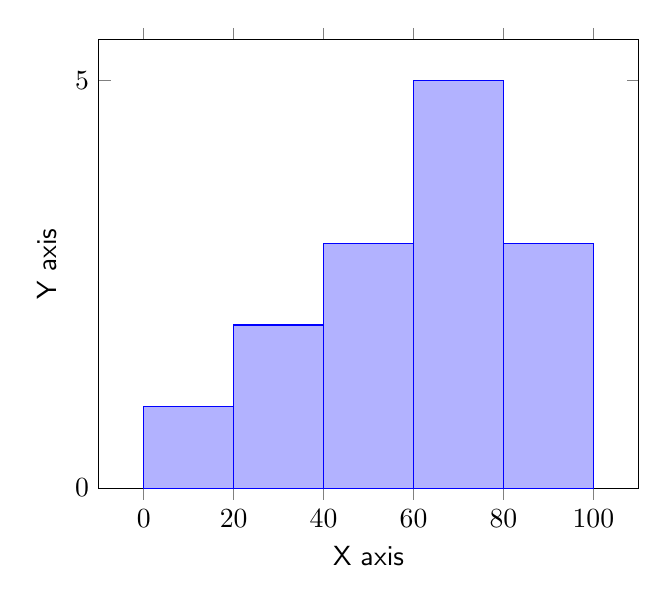
\begin{tikzpicture}
					\begin{axis}
					[
						ybar,
						ymin=0,
						xtick={0, 20, 40, 60, 80, 100},
						ytick={0, 5},
						xlabel=X axis,
						ylabel=Y axis
					]
						\addplot +
						[
							hist=
							{
								bins=5,
								data min=0,
								data max=100
							}
						] table [y index = 0]
						{
							10
							30
							30
							50
							50
							50
							70
							70
							70
							70
							70
							90
							90
							90
						};
					\end{axis}
				\end{tikzpicture}
				
				\caption{Example of a Distribution Skewed to the Left}
				\label{fig:distribution-skewed-to-the-left}
			\end{figure}
			
		&& \emph{Normal distribution:} Most data points are mainly in the centre of the distribution
			&&& Tails of data on the right and left; bulge of data in the centre
			&&& $median - Q1 \approx Q3 - median$
			&&& See subsection~\ref{subsec:analysis-of-single-variable-data:normal-distribution}
			&&& E.g. See figure~\ref{fig:distribution-normal}
			
			\begin{figure}[!htb]
				\centering
				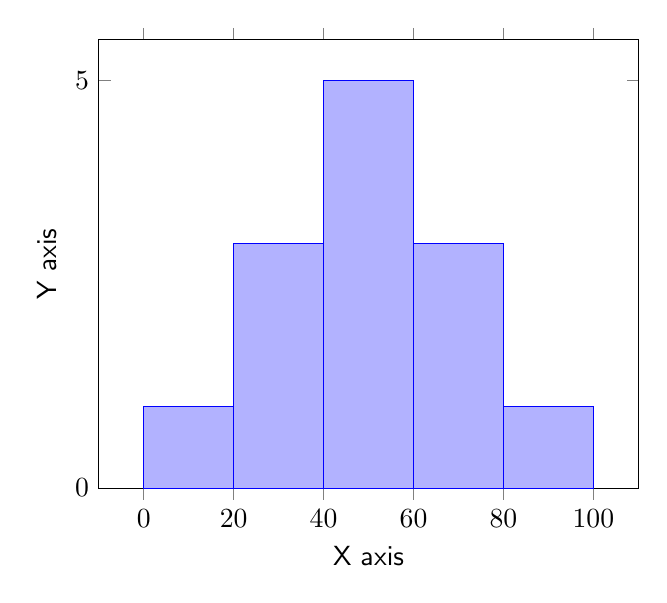
\begin{tikzpicture}[scale=1]
					\begin{axis}
					[
						ybar,
						ymin=0,
						xtick={0, 20, 40, 60, 80, 100},
						ytick={0, 5},
						xlabel=X axis,
						ylabel=Y axis
					]
						\addplot +
						[
							hist=
							{
								bins=5,
								data min=0,
								data max=100
							}
						] table [y index = 0]
						{
							10
							30
							30
							30
							50
							50
							50
							50
							50
							70
							70
							70
							90
						};
					\end{axis}
				\end{tikzpicture}
				
				\caption{Example of a Normal Distribution Skewed to the Right}
				\label{fig:distribution-normal}
			\end{figure}
			
		&& \emph{Skewed to the right:} Most data points are mainly on the left side of the distribution
			&&& Tail of data on the right; bulge of data on the left
			&&& $median - Q1 < Q3 - median$
			&&& E.g. See figure~\ref{fig:distribution-skewed-to-the-right}
			
			\begin{figure}[!htb]
				\centering
				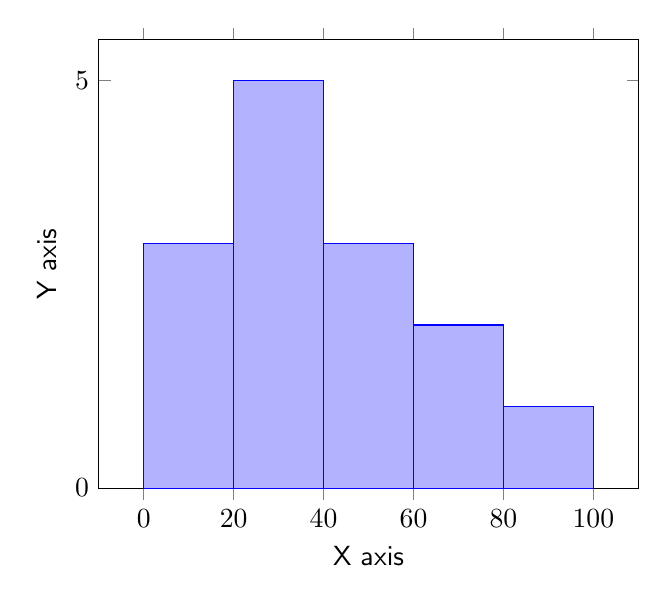
\begin{tikzpicture}[scale=1]
					\begin{axis}
					[
						ybar,
						ymin=0,
						xtick={0, 20, 40, 60, 80, 100},
						ytick={0, 5},
						xlabel=X axis,
						ylabel=Y axis
					]
						\addplot +
						[
							hist=
							{
								bins=5,
								data min=0,
								data max=100
							}
						] table [y index = 0]
						{
							10
							10
							10
							30
							30
							30
							30
							30
							50
							50
							50
							70
							70
							90
						};
					\end{axis}
				\end{tikzpicture}
				
				\caption{Example of a Distribution Skewed to the Right}
				\label{fig:distribution-skewed-to-the-right}
			\end{figure}
			
		&& Correspond directly to the boxplot
		&& Extreme values affect the mean more than the median:
			&&& Skewed to the left: Mean is less than the median
			&&& Normal distribution: Mean is roughly equal to the median
			&&& Skewed to the right: Mean is greater than the median
			
		\medskip
		&& E.g. The annual salary (in thousands) of 10 random UBC graduates was recorded and analyzed. See table~\ref{tab:ubc-graduates-five-number-summary} for the five-number summary.
		
		\Deactivate
		\begin{table}[!htb]
			\centering
			\caption{Five-Number Summary of UBC Graduates' Annual Salaries}
			\label{tab:ubc-graduates-five-number-summary}
			\begin{tabular}{ l r }
				Minimum & 16 \\
				Q1 & 25 \\
				Median & 30 \\
				Q3 & 42 \\
				Maximum & 80
			\end{tabular}
		\end{table}
		\Activate
		
		Median - Q1 = 30 - 25 = 5 \\
		Q3 - median = 42 - 30 = 12 \\
		Since the distance between the median and Q3 is greater than the distance between Q1 and the median, the distribution is skewed to the right.
		
		%TODO Weeks 1/2, Document 03, Page 3
				
	& \emph{Center:} Median of a distribution
		&& Used for general comparisons of magnitude
		
	& \emph{Spread/variability:} How data points are distributed across the range
		&& Often measured by IQR (see \emph{inter-quartile range}, subsection~\ref{subsec:analysis-of-single-variable-data:categorical-data})
			&&& The greater the IQR, the greater the spread
		&& Not often measured by range because it is affected greatly by outliers
			&&& Only used when a conclusion cannot be derived using the IQR

	& UBC study %TODO
	
	& E.g. Boxplot and summary statistics \smallskip \\ %TODO
	The shape is skewed to the right. \\
	The median exam score is 60\%. Therefore, about 50\% of students scored less than 60\%, while the other 50\% of students scored higher than 60\%. \\
	The spread: Ranges from 55\% min to 92\% max. The middle 50\% of exam scores are between 58\% at Q1 and 66.5\% at Q3. \\
	There are 2 outliers; therefore, 2 students received abnormally high exam scores.

	& \emph{Mean/Average:} Sum of a set of values divided by the number of values
		&& Denoted by an overline ($\overline{x}$)

	& \emph{Standard deviation:} 
		&& Denoted by $\sigma$
		&& Formula:
		\begin{displaymath}
		\sigma =
		\sqrt
		{
			\frac
			{
				\sum \limits_{i=0}^n (x_{i} - \overline{x})^2
			}
			{
				n - 1
			}
		}
		\end{displaymath}
		\Deactivate
		\begin{center}
			\begin{tabular}{ l r @{ = } l }
				where: & $x$ & variable data \\
				& $\overline{x}$ & mean of the variable data \\
				& $n$ & total number of sample data points
			\end{tabular}
		\end{center}
		\Activate
		
	& %TODO example, other
	
\end{easylist}
\subsection{Normal Distributions}
	\label{subsec:analysis-of-single-variable-data:normal-distribution}
\begin{easylist}

	& Use a mean and standard deviation to analyze a normal distribution
		
	& %TODO
	
	& \emph{Standard (z-) score:} 
		&& Formula: $z = \frac{x - mean}{s}$ %TODO LEGEND - s = standard deviation
			&&& $x = mean + z \cdot s$
		&& Shade the region of interest and use the standard normal table to find the corresponding percentage
			&&& Only calculate the z-score up to one significant digit
			&&& Standard normal table gives area to the left of the z-score; if the z-score is positive ( is greater than the mean), subtract it from 100\%
		&& Example: %TODO
	
\end{easylist}
\clearpage
	%
% STAT 100: Chance and Data Analysis - A Course Overview
% Section: Analysis of Multi-Variable Data
%
% Author: Jeffrey Leung
%

\section{Analysis of Multi-Variable Data}
	\label{sec:analysis-of-multi-variable-data}
\subsection{Relationships between Two Quantitative Variables}
	\label{subsec:analysis-of-multi-variable-data:relationships-between-two-quantitative-variables}
\begin{easylist}

	& Relationships between two quantitative variables:
	& \emph{Dependent/respondent variable:} Variable to be predicted
		&& Placed on the vertical (y) axis
	& \emph{Independent variable/predictor:} Variable used to predict the dependent variable
		&& Placed on the horizontal (x) axis
	& \emph{Scatterplot:} Visual comparisons of the values of two quantitative variables (see figure %TODO in bullet point?
	
	& \emph{positive/negative:}
	
	& Forms and strength of a relationship:
		&& \emph{Linear:} Approximate change in values can be summarized in a single 2-d direction
			&&& I.e. Points which follow a straight line
		&& \emph{Non-linear:} Values change in multiple 2-d directions
			&&& E.g. Exponential functions, trigonometric functions
			
		&& \emph{Strength:} Denseness of distribution which shows a clear form/relation
			&& 
		
	& \emph{Correlation coefficient:} Value which denotes the strength of the data
			&&& Denoted by $r$
			&&& Formula: $r = $
			&&& Value:
				&&&& $-1 \leq r \leq 1$
				&&&& Closer to -1, the data is more negatively related
				&&&& Closer to 0, the data is more weakly related 
				&&&& Closer to 1, the data is more positively related
			&&& Interpretation: The closer to 1 $r$ is, the stronger the correlation
			&&& Only applies to linear data
				&&&& 0 for non-linear data
			&&& Outliers may need to be removed before calculation
			&&& E.g. The correlation coefficient of a midterm grade and a final grade was found to be 0.8747. The relationship between the two grades is positive, strong, and linear.
			
		&& For an interpretation of the magnitude, see table~\ref{tab:strength-of-a-correlation-coefficient}
		
		\Deactivate
		\begin{table}[!htb]
			\centering
			\caption{Strength of a Correlation Coefficient}
			\label{tab:strength-of-a-correlation-coefficient}
			\begin{tabular}{ c l }
				Magnitude of the Correlation Coefficient & Strength \\
				\hline
				$0 < |r| < 0.4$ & Weak \\
				$0.4 \leq |r| < 0.6$ & Moderately weak \\
				$0.6 \leq |r| < 0.8$ & Moderately strong \\
				$0.8 \leq |r| < 1.0$ & Strong \\
				$|r| = 1$ & Perfect
			\end{tabular}
		\end{table}
		\Activate
		
		%TODO incomplete
				
			
	& Correlation:
		&& Declares an association between two variables
		&& Does not imply causation - i.e. an existing linear relationship does not mean a change in the independent variable causes a change in the dependent variable (see figure~\ref{fig:xkcd-552})
	
	\begin{figure}[!htb]
		\centering
		\caption{XKCD Webcomic - 552: Correlation}
		\label{fig:xkcd-552}
		\href{https://xkcd.com/552/}{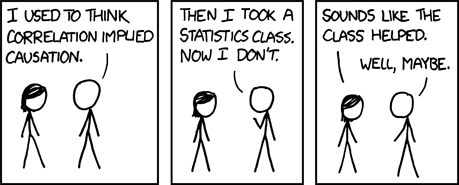
\includegraphics[scale=.75]{xkcd-552-correlation}}
	\end{figure}
		
		
	& \emph{Lurking variable:} Variable outside of the tested variables which explains an association between the two tested variables
		
	& \emph{Regression analysis:}
		&& \emph{Regression line:} Best-fit line
			&&& Before using the regression line to predict data, check data ranges
		&& %TODO
		&& \emph{Regression equation:} Mathematical equation of a regression line
			&&& May have multiple $x$ variables
			&&& Formula: $y = slope_1 \cdot x_1 + slope_2 \cdot x_2 + \ldots + slope_n \cdot x_n + y_{intercept}$
				&&&& Where $y =$ dependent variable, and $x_1, x_2, \ldots, x_n =$ independent variables
				&&&& Use a scientific calculator to determine the intercept and slope %TODO how
			&&& Cannot be used to predict data less than the minimum or greater than the maximum because there is no data to support the analysis
			&&& Slope of a regression equation: $\frac{y_{2} - y_{1}}{x_{2} - x_{1}}$
				&&&& Per 1 unit change in $x$, $y$ should change by the value of the slope
				&&&& Example of interp: For every 1 additional $x$, we predict $y$ will change by $slope$.
		&& \emph{Coefficient of determination:}
			&& Denoted by $R^{2}$
			&& Value:
				&&& $R^{2} = r^2$ where $r =$ the correltion coefficient
				&& $0 \leq R^{2} \leq 1$
			&& Interpretation: $R^{2}$ represents the variability in percent which can be explained by the regression line.
			%TODO notes
		
	& Multiple regression:
		&& See video
		&& Use excel
		
	
		
\end{easylist}
\clearpage
	%
% STAT 100: Chance and Data Analysis - A Course Overview
% Section: Data Collection
%
% Author: Jeffrey Leung
%

\section{Data Collection}
	\label{sec:data-collection}
\subsection{Methods}
	\label{subsec:data-collection:methods}
\begin{easylist}

	& \emph{Census:} Survey which collects information from all individuals of a population
		&& Process important?
		&& Not always viable because it may be:
			&&& Expensive
			&&& Time-consuming
			&&& Impossible (e.g. taking a census of everyone in the world)
		&& E.g. Taking a census of all Canadian citizens
		
	& \emph{Sample survey:} Survey which collects information from a select group of individuals smaller than and representative of the population
		&& Relatively greater data quality due to smaller samples
		&& E.g. Taking a sample survey of which political party for which people plan to vote
		
	& \emph{Observational study:} Data collection method in which data is collected through observation without interference
		&& Concludes an correlation or lack thereof between two variables
			&&& Lurking variable(s) (see ref) may connect the two variables and explain the association %TODO reference
		%TODO
		&& E.g. Students were given the option to attend an optional tutorial session. Those who attended the tutorial session were more likely to receive a higher mark on their exam. %TODO
	
	& \emph{(Randomized) Experiment:} Data collection method in which individuals are chosen randomly to... %TODO
		&& Not all factors can be studied through randomized experiments
		&& E.g. Some students are chosen at random to be given extra tutorial sessions. They receive...
		%TODO
		
		%TODO references to the subsections below

\end{easylist}
\subsection{Sampling}
	\label{subsec:data-collection:sampling}
\begin{easylist}

	& \emph{Random sample:} %TODO
	
	& \emph{Simple random sample:} Set of individuals selected from the population such that each individual has an equal chance of being selected
		&& Process: To select $y$ individuals from a group of $x$, number each individual
		&& %TODO
		
\end{easylist}
\subsection{Sampling Errors}
	\label{subsec:data-collection:sampling-errors}
\begin{easylist}

	& Non-sample errors:
	
		&& \emph{Response error:} Inaccurate/untruthful response which skews data
			&&& E.g. An experiment which asks a question about a morally shameful activity may have a response error due a tendency to answer with the morally best choice, so as to give a better impression
		&& \emph{Non-response error:} Lack of response which skews data
			&&& E.g. An experiment which offers an optional response to a survey, such as through email, may have a non-response error due to some people not responding because of not checking email, laziness, apathy
			&&& No standard way to determine a good response rate
				&&&& Theoretically, 75\% and above is acceptable
			&&& Analyze the response rate if possible, and the reason for a low response rate
		&& \emph{Question wording:} Syntax/keywords/details of a question in a survey which skews data
		
	& Voluntary response error:
		&& To explain, calculate the (low) response rate and offer a possible explanation

\end{easylist}
\subsection{Design of an Experiment}
	\label{subsec:data-collection:design-of-an-experiment}
\begin{easylist}

	& \emph{Explanatory variable:} Factor which is hypothesized to affect another factor
		&& \emph{Treatment:} Unique combination of one of each type of explanatory variable
			&&& $Number\ of\ treatments = num\ of\ variable_{1} \times num\ of\ variable_{2} \times \cdots$
			&&& Table of all possible treatments should be written
			&&& Sample is assigned equally and randomly into the number of treatments
	& \emph{Response variable:} Resultant factor which is hypothesized to be affected by another factor
	
	& Experiment diagram + block diagram %TODO
	
	& E.g. An experiment was conducted to find out if the length and/or repetitions of a TV commercial affect the desire to buy a product. 20 subjects were chosen for the experiment. \smallskip \\
	
	\emph{Explanatory variables:} \\
	\indent Length of the TV commercial (1 minute / 5 minutes / 10 minutes) \\
	\indent Number of repetitions of the TV commercial (1 time / 3 times / 5 times) \\
	\emph{Response variable:} \\
	Desire to buy the product in the TV commercial (Scale from 1-5 where 1 = Do not want to buy) \\
	\emph{Treatments:} \\
	$3 \times 3 = 9$ treatments (see table~\ref{tab:experiment-length-repetitions-commercial-treatments}) \\
	
	
	
	\Deactivate
	\begin{table}[!htb]
		\centering
		\caption{Treatments of a Experiment on Length and Repetitions of a Commercial}
		\label{tab:experiment-length-repetitions-commercial-treatments}
		\begin{tabular}{ r r }
			Length (mins): & Repetitions: \\
			\hline
			 1 & 1 \\
			   & 3 \\
			   & 5 \\
			 5 & 1 \\
			   & 3 \\
			   & 5 \\
			10 & 1 \\
			   & 3 \\
			   & 5
		\end{tabular}
	\end{table}
	\Activate
		
\end{easylist}
\clearpage
	%
% STAT 100: Chance and Data Analysis - A Course Overview
% Section: Analysis of Population Proportions
%
% Author: Jeffrey Leung
%

\section{Analysis of Population Proportions}
	\label{sec:analysis-of-population-proportions}
\subsection{Margin of Error and Confidence Interval}
	\label{subsec:analysis-of-population-proportions:margin-of-error-and-confidence-interval}
\begin{easylist}

	& \emph{Parameter:} Value which summarizes population data
		&& Calculation requires collection of data from the entire population (i.e. see \emph{census}, subsection~\ref{subsec:data-collection:methods})
		&& Estimation is often calculated from a sample statistic
			&&& E.g. If 33\% of a random sample of Canadian adults support the Conservative Party, then the proportion of all Canadian adults who support the Conservative Party is estimated to be 33\%.
		&& Denoted by $p$
			&&& Sample proportion/statistic is denoted by $\hat{p}$
	
	\medskip
	& \emph{Margin of error:} Percentage value of the uncertainty of an estimated population proportion
		&& Calculation (for a 95\% confidence level):
		\begin{math}
			Margin\ of\ error = \frac{1}{\sqrt{sample\ size}}
		\end{math}
			&&& Unit: Percentage
		&& Valid only for a random sample
		&& Dependent on a confidence level
			&&& \emph{Confidence level:} Degree of certainty of the accuracy of a population proportion estimate
				&&&& Unit: Percentage
				&&&& Often 95\% (expressed as a fraction; 19 times out of 20 = $\frac{19}{20}$)
		&& Interpretation (with the confidence level): \smallskip \\
		If many random samples of <sample size, subject> of the population are taken and the sample proportion of <statistic> is calculated for each sample, <confidence level percentage> of the sample proportions will be within $\pm$ <margin of error percentage> of the population proportion.
		
		&& E.g. ``A probability sample of this design and sample size would carry a margin of error in the range of $\pm 1.2\%$, 19 times out of 20.'' \smallskip \\
		Margin of error: $\pm 1.2\%$ \\
		Confidence level: $\frac{19}{20} = 95\%$
		&& E.g. Given a study of Canadian adults who support the Conservatives with a random sample of 6005 Canadian adults and a margin of error of $\pm$ 1.2\%, 19 times out of 20: \smallskip \\
		If many random samples of 6005 Canadian adults of the population are taken and the sample proportion of Canadian adults who support the Conservatives is calculated for each sample, 95\% of the sample proportions will be within $\pm$ 1.2\% of the population proportion.
	
	\medskip
	& \emph{Confidence interval:} Set of values which the population proportion is within
		&& Calculation:
		\begin{math}
			Confidence\ interval = sample\ proportion \pm margin\ of\ error
		\end{math}
			&&& Unit: Percentage range
		&& Interpretation: \smallskip \\
		Using the sample data, we are <confidence level percentage> confident that the population proportion of <statistic> is between <confidence interval lower bound percentage> and <confidence interval upper bound percentage>.
			&&& Always specify the population proportion
		&& E.g. Given the sample proportion of Canadian adults who will vote for the Conservatives as 33\% for 6005 subjects, the confidence interval is: \\
		\begin{math}
			Sample\ proportion \pm \frac{1}{\sqrt{sample\ size}}
			= 33\% \pm \frac{1}{\sqrt{6005}}
			= 33\% \pm 1.2904...\%
			\approx (31.7\%, 34.3\%)
		\end{math} \\
		Using the sample data, we are 95\% confident that the population proportion of Canadian adults who support the Conservative Party is between 31.7\% and 34.3\%.
		
		&& Analyzing the confidence interval: Given a value, check whether or not all values of the confidence interval satisfy the condition
			&&& E.g. Given the confidence interval for the population proportion of Canadian adults who support the Conservative Party to be (31.7\%, 34.3\%), can you conclude that more than 30\% of all Canadian adults support the Conservative Party? \smallskip \\
			Yes; all values in the confidence interval are greater than 30\%.
			&&& E.g. Given the confidence interval for the population proportion of Canadian adults who support the Conservative Party to be (31.7\%, 34.3\%), can you conclude that more than 34\% of all Canadian adults support the Conservative Party? \smallskip \\
			No; there exist values in the confidence interval which are less than 34\%.
			
\end{easylist}
\subsection{Bias and Variability}
	\label{subsec:analysis-of-population-proportions:bias-and-variability}
\begin{easylist}

	& \emph{Bias:} Consistent under-estimation or over-estimation of results
		&& Can be reduced by:
			&&& Avoiding \hyperref[subsec:data-collection:sampling-errors]{non-sampling errors}
			&&& Ensuring fair representation of the population
			&&& Using random sampling
		&& Increasing sample size does not reduce bias
			
	& \emph{Sampling variability:} Degree of variability between random samples
		&& Quantified by the \hyperref[subsec:analysis-of-population-proportions:margin-of-error-and-confidence-interval]{margin of error}
		&& Can be reduced by:
			&&& Increasing sample size
			
\end{easylist}
\subsection{Hypothesis Testing for Population Proportions}  %TODO move this to a different file
	\label{subsec:analysis-of-population-proportions:hypothesis-testing-for-population-proportions}
\subsubsection{Introduction}
	\label{subsubsec:analysis-of-population-proportions:hypothesis-testing-for-population-proportions:introduction}
\begin{easylist}

	& \emph{Hypothesis test:} Calculation which determines whether a claim/research hypothesis is supported by evidence

	& \emph{Null hypothesis (H\textsubscript{o}):} Statement that a population proportion is equal to a given value (which may be another population proportion)
		&& Assumed to be possible until contradicting evidence is found
	& \emph{Alternative hypothesis (H\textsubscript{a}):} Statement that a population proportion is less than, not equal to, or greater than a given value (which may be another population proportion)
	& E.g. The sample proportion of Canadian adults who want to legalize marijuana was found to be 59\%. Test whether or not the population proportion of Canadian adults who want to legalize marijuana is greater than 50\%. \\
	H\textsubscript{o}: The population proportion of Canadian adults who want to legalize marijuana is equal to 50\%. \\
	H\textsubscript{a}: The population proportion of Canadian adults who want to legalize marijuana is greater than 50\%.
	
	\medskip
	& \emph{Test statistic:} Standardized value representing a numerical summary of sample data 
		&& Calculated from sample data; analyzed to determine the p-value
		&& E.g. Z-statistic, t-statistic, chi-square statistic
		&& \emph{Z-statistic:} Test statistic which can be calculated to determine whether an inequal relationship between population proportions exists
			&&& Formula for one population proportion compared against a given percentage: \smallskip \\
			\begin{displaymath}
				z-statistic = 
				\frac
				{
					\hat{p} - p_{0}
				}
				{
					\sqrt
					{
						\frac
						{
							p_{0} \cdot (1 - p_{0})
						}
						{
							n
						}
					}
				}
			\end{displaymath}
			\Deactivate
			\begin{center}
				\begin{tabular}{ l r @{ = } l }
					where & $\hat{p}$ & sample proportion \\
					& $p_{0}$ & population proportion if H\textsubscript{0} is true \\
					& $n$ & sample size
				\end{tabular}
			\end{center}
			\Activate
			
			\medskip
			&&& Formula for two population proportions compared against each other: \medskip \\
			\begin{displaymath}
				z-statistic =
				\frac
				{
					\hat{p_{1}} - \hat{p_{2}}
				}
				{
					\sqrt
					{
						\hat{p} \cdot (1-\hat{p}) \cdot
						(
							\frac{1}{n_{1}} + \frac{1}{n_{2}}
						)
					}
				}
			\end{displaymath}
			\Deactivate
			\begin{center}
				\begin{tabular}{ l r @{ = } l }
					where & $\hat{p_{x}}$ & sample proportion of the $x$\textsuperscript{th} set of data \\
					& $\hat{p}$ & combined sample proportion \\
					& $n_{x}$ & sample size of the $x$\textsuperscript{th} set of data
				\end{tabular}
			\end{center}
			\Activate
			
				&&&& Combined sample proportion is the sum of the number of subjects satisfying the condition of sample dataset 1 and the number of subjects satisfying the condition of sample dataset 2, divided by the sum of the number of subjects of each dataset
			
		&& \emph{Chi-square statistic:} %TODO
	
	\medskip
	& \emph{Probability value (p-value):} Probability that a given result is obtained through chance, calculated from sample data
		&& Unit: Percentage
		&& Interpretation: If many random samples of the given sample size and population are chosen and the sample proportion in question is calculated, then the p-value represents the percentage of the sample populations which would support the alternative hypothesis.
			&&& E.g. Given that 50\% of all Canadian adults support the legalization of marijuana, the probability of calculating a sample proportion of 59\% or higher through random sampling is equal to the p-value (0.62\%).
		&& The lesser the p-value, the greater the evidence for the alternative hypothesis
		&& Calculated from a test statistic; compared against the significance level to determine the amount of evidence for the alternative hypothesis
		&& For the interpretation of the p-value compared against the significance level, see \hyperref[subsec:analysis-of-population-proportions:statistical-significance]{statistical significance}
		&& For the interpretation of the magnitude, see table~\ref{tab:p-value-magnitude-chart}
		
		\Deactivate
		\begin{table}[!htb]
			\centering
			\caption{P-Value Magnitude Chart}
			\label{tab:p-value-magnitude-chart}
			\begin{tabular}{ r c l l }
				\multicolumn{3}{ c }{P-value} & Strength of Evidence to Support H\textsubscript{a} \\
				 10\% < & p-value & & No evidence \\
				  5\% < & p-value & $\leq$  10\% & Weak evidence \\
				  1\% < & p-value & $\leq$   5\% & Some evidence \\
				0.1\% < & p-value & $\leq$   1\% & Strong evidence \\
				        & p-value & $\leq$ 0.1\% & Very strong evidence
			\end{tabular}
		\end{table}
		\Activate
		
		&& P-value of a z-statistic: Area under the standard normal distribution where z-statistic equals the z-score (see %\ref standard normal table
			&&& If the alternative hypothesis is `less than', the p-value is the area to the left of the z-statistic
			&&& If the alternative hypothesis is `not equal to', the p-value is the area to the left of the negative absolute value of the z-statistic an the area to the right of the positive absolute value of the z-statistic
			&&& If the alternative hypothesis is `greater than', the p-value is the area to the right of the z-statistic
		&& P-value of a chi-square statistic: %TODO
		
	& \emph{Significance level:} %TODO
			
	& General process:
		&& Find the test statistic using the sample data
		&& Find the p-value using the test statistic
		&& Compare the p-value to the significance level
			&&& Conclusion: ``Since the p-value (<p-value>) is <less than/greater than> the significance level (<significance level>), we <do not> reject the null hypothesis. There is <sufficient/insufficient> evidence to conclude that <alternative hypothesis>.''

\end{easylist}
\subsection{One Population Proportion (Z-Statistic)}
	\label{subsec:analysis-of-population-proportions:one-population-proportion-z-statistic}
\begin{easylist}
	
	& 
	& E.g. %TODO

\end{easylist}
\subsection{Two Population Proportions (Z-statistic)}
	\label{subsec:analysis-of-population-proportions:two-population-proportions-z-statistic}
\begin{easylist}

	& Process:
		&& Compute the proportion of subjects in each test group who satisfy the condition
		&& Compare the proportions using a bar graph
		&& Conclude which group has a greater/lesser proportion
		&& To compare population proportions, conduct a hypothesis test (see %TODO ref
			&&& Null hypothesis states that the population proportions are equal; alternative hypothesis states that the population proportions are unequal (less than, not equal to, or greater than)
			&&& Formula for the z-statistic for two population proportions:
		
	& E.g. Are the proportions...
	
\end{easylist}
\subsubsection{Confidence Interval}
	\label{subsubsec:analysis-of-population-proportions:two-population-proportions-z-statistic:confidence-interval}
\begin{easylist}

	& Formula (95\% confidence interval):
	\begin{math}
		(\hat{p_{1}} - \hat{p_{2}}) \pm 2 \cdot
		\sqrt
		{
			\frac
			{
				\hat{p_{1}} \cdot (1 - \hat{p_{1}})
			}{
				n_{1}
			}
			+ \frac
			{
				\hat{p_{2}} \cdot (1-\hat{p_{2}})
			}{
				n_{2}
			}
		}
	\end{math}
	
	& Example: [..] How does the proportion of people who have lung cancer...
	
	& There may be no difference between the proportion of students who use iPhones in UBC compared to the proportion of students who use iPhones in SFU.
	
\end{easylist}
\subsection{Multiple Population Proportions (Chi-Square Statistic)}
	\label{subsec:analysis-of-population-proportions:multiple-population-proportions-chi-square-statistic}
\begin{easylist}

	& The greater the difference, the greater the chi-square statistic
	& P-value always uses the right side of the normal distribution
	& Only concludes whether a relationship exists between two variables
	& Can compare many population proportions

\end{easylist}
\subsection{Errors}
	\label{subsec:analysis-of-population-proportions:errors}
\begin{easylist}

	& \emph{Type I error:} Rejection of H\textsubscript{o} from analysis of the sample data when H\textsubscript{o} is true
		&& I.e. False positive/confirmation of the alternative hypothesis; finding evidence where there is none
		&& May occur when H\textsubscript{o} is rejected
		&& E.g. Judging a person for a crime: \\
		H\textsubscript{o}: The person is not guilty. \\
		H\textsubscript{a}: The person is guilty. \\
		Truth: The person is not guilty (H\textsubscript{o} is true). \\
		Decision: The person is guilty (H\textsubscript{o} is rejected).
		&& Probability of its occurrence is directly proportional to the \hyperref[subsubsec:analysis-of-population-proportions:hypothesis-testing-for-population-proportions:introduction]{significance level}
			&&& Reducing significance level (and therefore, the probability of the type I error) increases the probability of the type II error
		
	& \emph{Type II error:} Failure to reject H\textsubscript{o} from analysis of the sample data when H\textsubscript{a} is true
		&& I.e. Failing to find evidence which exists
		&& May occur when H\textsubscript{o} is not rejected
		&& E.g. Judging a person for a crime: \\
		H\textsubscript{o}: The person is not guilty. \\
		H\textsubscript{a}: The person is guilty. \\
		Truth: The person is guilty (H\textsubscript{a} is true). \\
		Decision: The person is not guilty (H\textsubscript{o} is not rejected).
		&& Probability of its occurrence is inversely proportional to the \hyperref[subsubsec:analysis-of-population-proportions:hypothesis-testing-for-population-proportions:introduction]{significance level}
			&&& Increasing significance level (and therefore, the probability of the type II error) increases the probability of the type I error
			
	& E.g. A company will renew a contract with a radio station only if the station can find sufficient evidence to support that more than 20\% of the listeners have heard their ad. The station conducts a random survey of 400 people, 100 of which have heard the ad. \smallskip \\
	H\textsubscript{o}: 20\% of the listeners have heard the ad. \\
	H\textsubscript{a}: More than 20\% of the listeners have heard the ad. \smallskip \\
	A type I error will occur if 20\% of the listeners have heard the ad, but the sample data provides sufficient evidence to conclude that more than 20\% of the listeners have heard the ad. H\textsubscript{o} is true but rejected; H\textsubscript{a} is false but accepted. \\
	The possibility of this error can be reduced by decreasing the significance level. \smallskip \\
	A type II error will occur if more than 20\$ of the listeners have heard the ad, but the sample data does not provide sufficient evidence to reject the hypothesis that 20\% of the listeners have heard the ad. H\textsubscript{o} false but not rejected; H\textsubscript{a} is true but not affirmed. \\
	The possibility of this error can be reduced by increasing the significance level.
	
\end{easylist}
\subsection{Statistical Significance}
	\label{subsec:analysis-of-population-proportions:statistical-significance}
\begin{easylist}

	& P-value represents the probability that a given sample proportion is found, if the null hypothesis is correct, and therefore the probability of obtaining a difference of | sample proportion - test proportion | from the test proportion
	
	& \emph{Statistically significant:} Result which is unlikely to occur by chance
		&& Statistically significant result: P-value is less than the significance level
		&& Not statistically significant result: P-value is greater than the significance level
	
	& If a p-value is less than the significance level, then the difference between the sample proportion and the test proportion is statistically significant at the given significance level
	& If a p-value is greater than the significance level, then the difference between the sample proportion and the test proportion is not statistically significant at the given significance level


\end{easylist}
\clearpage
	%%
% STAT 100: Chance and Data Analysis - A Course Overview
% Section: Probability
%
% Author: Jeffrey Leung
%

\section{Probability}
	\label{sec:probability}
\subsection{Introduction}
	\label{subsec:probability:introduction}
\begin{easylist}

	& \emph{Experiment:} Process which creates a bag of outcomes
	& \emph{Sample space:} Set of all possible outcomes
		&& Denoted by $S$
	& \emph{Event:} Possible outcome which satisfies a given condition(s)
		&& Denoted by $E$

	& \emph{Probability:} Value between 0 and 1 (inclusive) representing the proportion of times an outcome/event is expected
		&& Denoted by $P(event)$
		&& Calculation:
		\begin{math}
			P(A) = \frac{|A|}{|S|}
		\end{math}
		where |X| is the number of outcomes for X
		&& 0 means the event is impossible; 1 means the event is certain
		&& Represented either by a fraction or a decimal value
		
		&& E.g. The probability of getting an odd number when rolling a 6-sided die:
		
		\medskip
		\Deactivate
		\begin{center}
			\begin{tabular}{ r @{ = } l }
				$S$ & Results of rolling a 6-sided die = 1, 2, 3, 4, 5, 6 \\
				$|S|$ & 6 \\
				$E$ & Getting an odd number = 1, 3, 5 \\
				$|E|$ & 3 \\
				$P(E)$ & $\frac{|E|}{|S|}$ = $\frac{3}{6}$ = 0.5
			\end{tabular}
			\Activate
		\end{center}
		
	& %TODO


\end{easylist}
\clearpage
	%
% STAT 100: Chance and Data Analysis - A Course Overview
% Section: Measurement of Data
%
% Author: Jeffrey Leung
%

\section{Measurement of Data}
	\label{sec:measurement-of-data}
\subsection{Introduction}
	\label{subsec:measurement-of-data:introduction}
\begin{easylist}

	& \emph{Measurement:} Collection of quantitative data
	
	& \emph{Unit of measurement:} System of set values to quantify data
		&& Comparisons between measurements must use the same units
	
	& \emph{Instrument:} Tool to measure a quantitative characteristic of an individual
		&& E.g. Ruler, scale
		
\end{easylist}
\subsection{Imprecision of Measurements}
	\label{subsec:measurement-of-data:imprecision-of-measurements}
\begin{easylist}

	& \emph{Uncertainty (measurement):} Possible error in a measurement due to imprecision of an instrument
	& \emph{Bias (measurement):} Difference between the measured value and the true value of a quantitative characteristic
	& Uncertainty and bias can be reduced by using instruments with higher precision

	& \emph{Random error:} Variations between repeated measurements on the same individual
		&& E.g. Surveying 100 people out of a population of 1000; recording the weight of a live, energetic pig
		&& Can be reduced by averaging multiple repeated measurements
		&& The less the random error, the more reliable the measurement
		
	& \emph{Variance:} Unreliability of a measurement (calculated from multiple measurements
		&& Calculation:
		\begin{displaymath}
			Variance =
			\frac
			{
				\sum\limits_{i=0}^{n}
				(x_{i} - \bar{x})^{2}
			}
			{
				n - 1
			}
		\end{displaymath}
		\Deactivate
		\begin{center}
			\begin{tabular}{ l r @{ = } l }
				where & $n$ & number of measurements \\
				& $x_{i}$ & measurement number $i$ \\
				& $\bar{x}$ & average of measurements
			\end{tabular}
		\end{center}
		\Activate
		
		&& E.g. Find the variance of the measurements 220 lbs, 224 lbs, 217 lbs, and 227 lbs.
		
		\Deactivate
		\begin{center}
			\begin{tabular}{ r @{ = } l }
				$n$ & 4 \\
				$\bar{x}$ & $\frac{220 + 224 + 217 + 227}{4} = \frac{888}{4} = 222$
			\end{tabular}
		\end{center}
		\Activate
		
		\Deactivate
		\begin{IEEEeqnarray}{ r C l }
			Variance
			& = & \frac
			{
				\sum\limits_{i=0}^{n}
				(x_{i} - \bar{x})^{2}
			}
			{
				n - 1
			} \\
			& = & \frac
			{
				(220-222)^{2} + (224-222)^{2} + (217-222)^{2} + (227-222)^{2}
			}
			{
				4-1
			} \\
			& = & \frac
			{
				4 + 4 + 25 + 25
			}
			{
				3
			} \\
			& = & \frac{58}{3}
		\end{IEEEeqnarray}
		\Activate

\end{easylist}
\subsection{Relevancy of a Measurement}
	\label{subsec:measurement-of-data:relevancy-of-a-measurement}
\begin{easylist}

	& A valid measurement should be a relevant representation of the property to be studied, and not some other property

	& Rates are a standard measure of comparison, while counts are not
		&& E.g. Out of 50 people, the morning class had 20 attendees. Out of 100 people, the evening class had 30 attendees. \smallskip \\
		Comparing the number/count of subjects, the evening class (30) had greater attendance than the morning class (20). \\
		Comparing the rates of subjects, the morning class ($\frac{20}{50} = 0.4$) had greater attendance than the evening class ($\frac{30}{100} = 0.3$).

\end{easylist}
\clearpage
	%
% STAT 100: Chance and Data Analysis - A Course Overview
% Section: Ethics
%
% Author: Jeffrey Leung
%

\section{Ethics}
	\label{sec:ethics}
\begin{easylist}

	& Standard ethical procedures:
		&& \emph{Institutional review board:} Group which judges whether a study will provide valuable information and is statistically sound
		&& Having an institutional review board ensure that subjects are not harmed
		&& Collecting assurance of informed consent in advance from all subjects
			&&& Information about the nature, purpose, and possible risks of the study
			&&& Not required only when it concerns observation in a public area
		&& Prevention of any possible physical harm
		&& Keeping all data confidential and anonymous
		
	& Other considerations:
		&& Emotional harm
		&& Privacy
		&& Deception

	& Examples of unethical procedures:
		&& Selling products under the guise of conducting a survey
		&& Publishing fabricated data
		
	& \emph{Clinical trial:} Experiment which studies the effects of various medical treatments on human patients
		&& Risks for the current experimental patients; benefits for future patients
		&& Random comparative experiments ensure the real effects of a treatment are shown
		&& Medical ethics and international ethics support the interests of the subject over the interests of the society
			&&& Therefore, there is only reason to conduct clinical trials when there is:
				&&&& Sufficient reason to believe the treatment may help the experimental group
				&&&& Sufficient doubt to believe the treatment may help the control group
				

\end{easylist}
\clearpage
	
\end{document}